% Approved CritiCal system overview: direction A (parallel evidence paths).
% Native TikZ; see input-example-provenance.txt for illustrative thumbnail source.
\begingroup
\definecolor{criticalEFF5F9}{HTML}{EFF5F9}
\definecolor{criticalC7D0D6}{HTML}{C7D0D6}
\definecolor{critical246083}{HTML}{246083}
\definecolor{criticalEEF6F2}{HTML}{EEF6F2}
\definecolor{critical23675B}{HTML}{23675B}
\definecolor{criticalF7F8FA}{HTML}{F7F8FA}
\definecolor{critical202830}{HTML}{202830}
\definecolor{criticalFFFFFF}{HTML}{FFFFFF}
\definecolor{critical56616B}{HTML}{56616B}
\definecolor{critical8A5824}{HTML}{8A5824}
\resizebox{0.84\textwidth}{!}{%
\begin{tikzpicture}[x=1pt,y=-1pt]
\path[use as bounding box] (0,20) rectangle (1440,558);
\path[fill=criticalEFF5F9,draw=criticalC7D0D6,line width=1.6pt,rounded corners=8pt] (230,22.5) rectangle (730,247.5);
\node[anchor=base west,inner sep=0pt,outer sep=0pt,text=critical246083,font={\sffamily\fontsize{25}{30.5}\selectfont\bfseries}] at (248,53.1) {1  Diverse-perceiver measurement};
\path[fill=criticalEEF6F2,draw=criticalC7D0D6,line width=1.6pt,rounded corners=8pt] (230,297) rectangle (730,499.5);
\node[anchor=base west,inner sep=0pt,outer sep=0pt,text=critical23675B,font={\sffamily\fontsize{25}{30.5}\selectfont\bfseries}] at (248,327.6) {2  Adversarial feature discovery};
\path[fill=criticalF7F8FA,draw=criticalC7D0D6,line width=1.6pt,rounded corners=8pt] (755,22.5) rectangle (1420,499.5);
\node[anchor=base west,inner sep=0pt,outer sep=0pt,text=critical202830,font={\sffamily\fontsize{25}{30.5}\selectfont\bfseries}] at (773,53.1) {3  Calibrated decision routing};
% Concrete input example; the two AI-generated halves are clipped natively.
\path[fill=criticalFFFFFF,draw=critical202830,line width=1.6pt,rounded corners=5pt] (15,96) rectangle (180,526);
\node[anchor=base,inner sep=0pt,outer sep=0pt,text=critical202830,font={\sffamily\fontsize{22}{26.84}\selectfont\bfseries}] at (97.5,129) {Instruction};
\node[anchor=base,inner sep=0pt,outer sep=0pt,text=critical202830,font={\sffamily\fontsize{20}{24.4}\selectfont}] at (97.5,156) {Show pink-dress};
\node[anchor=base,inner sep=0pt,outer sep=0pt,text=critical202830,font={\sffamily\fontsize{20}{24.4}\selectfont}] at (97.5,180) {making in steps.};
\node[anchor=base west,inner sep=0pt,outer sep=0pt,text=critical202830,font={\sffamily\fontsize{21}{25.62}\selectfont\bfseries}] at (25,211) {Video A};
\begin{scope}
\clip (25,224) rectangle (170,332.75);
\node[anchor=north west,inner sep=0pt,outer sep=0pt] at (25,224) {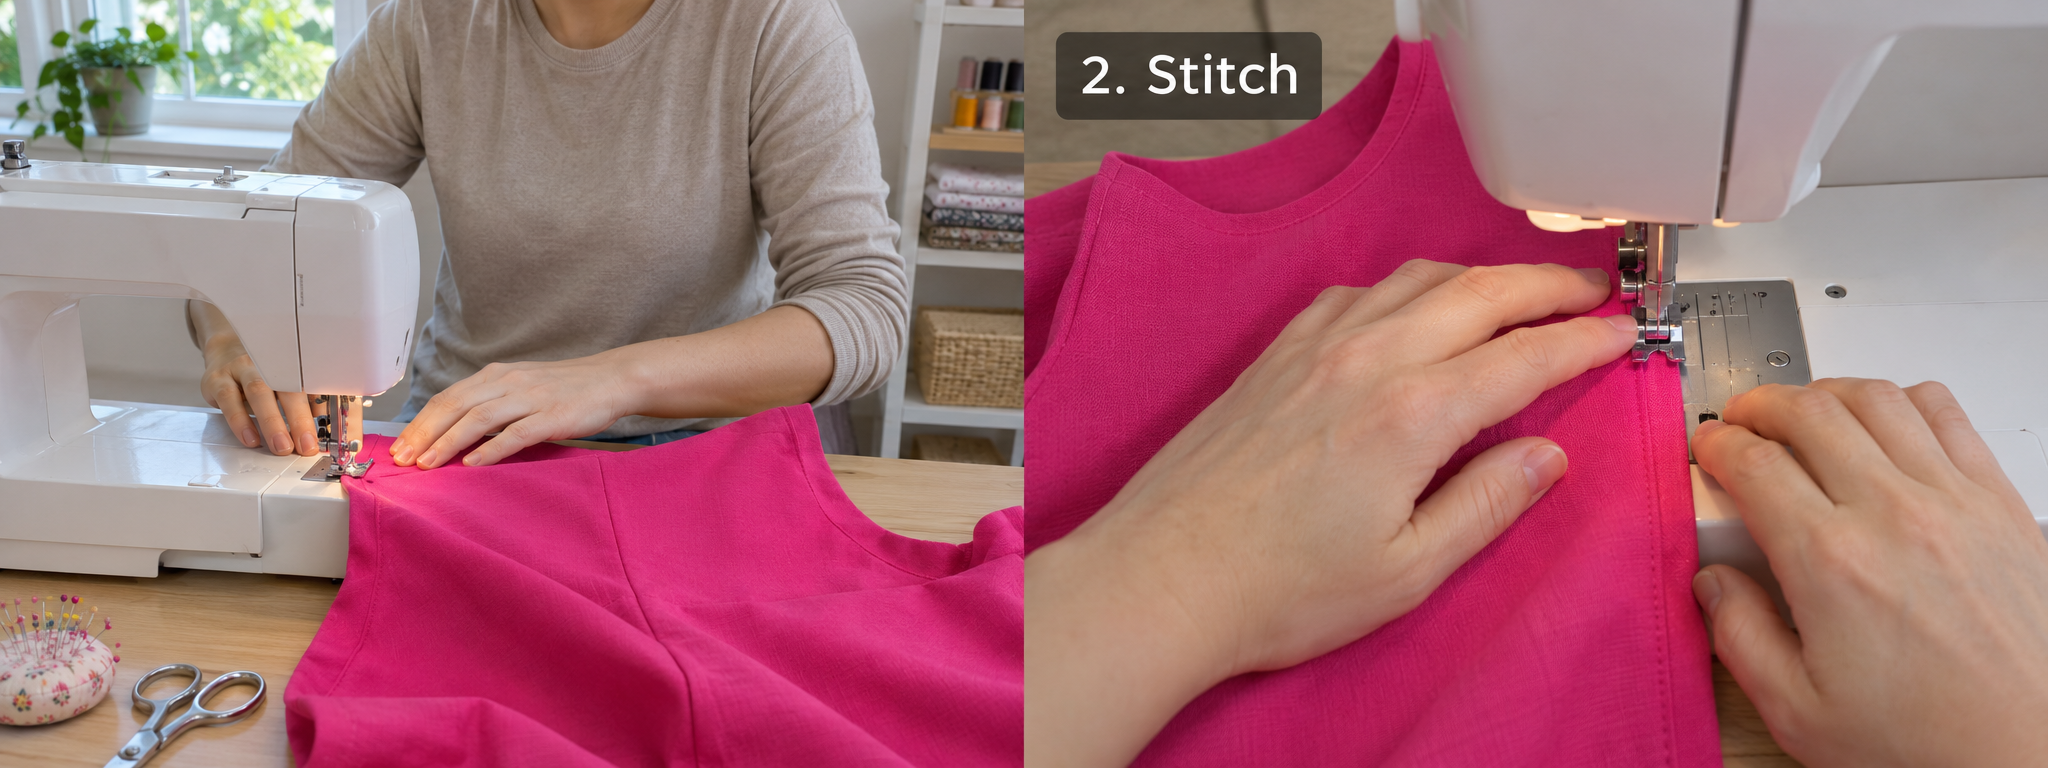
\includegraphics[width=290pt]{figures/flowchart/input-example-pair.png}};
\end{scope}
\node[anchor=base west,inner sep=0pt,outer sep=0pt,text=critical202830,font={\sffamily\fontsize{21}{25.62}\selectfont\bfseries}] at (25,357) {Video B};
\begin{scope}
\clip (25,370) rectangle (170,478.75);
\node[anchor=north west,inner sep=0pt,outer sep=0pt] at (-120,370) {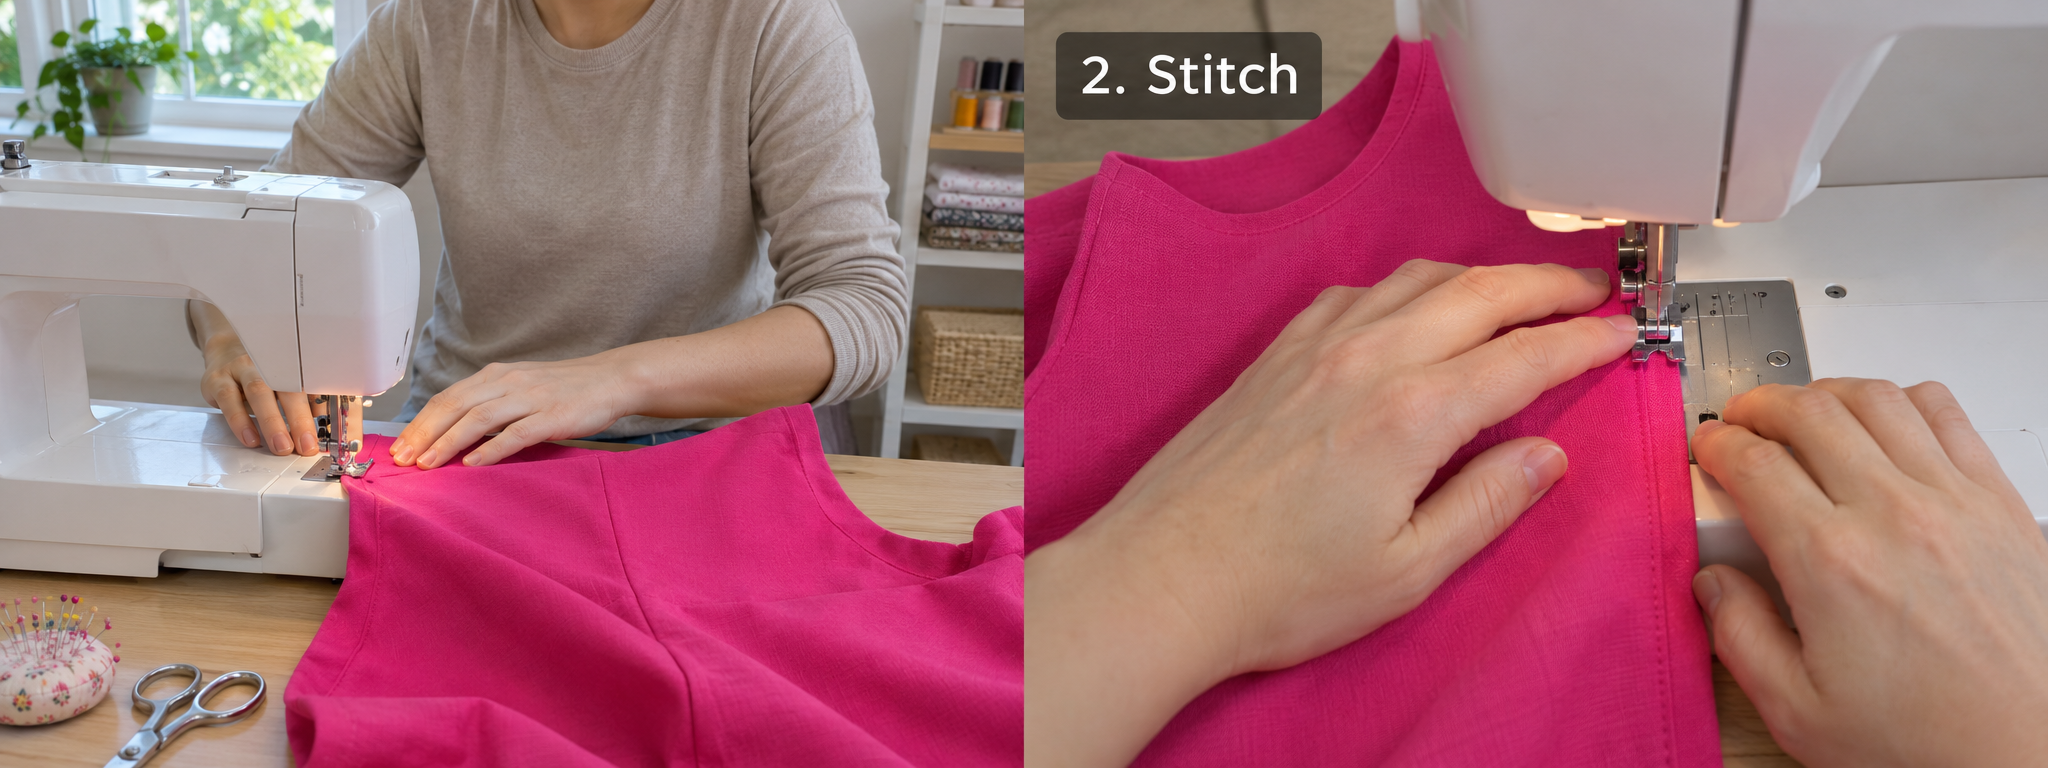
\includegraphics[width=290pt]{figures/flowchart/input-example-pair.png}};
\end{scope}
\node[anchor=base,inner sep=0pt,outer sep=0pt,text=critical56616B,font={\sffamily\fontsize{20}{24.4}\selectfont}] at (97.5,511) {Illustrative frames};
\draw[draw=critical202830,line width=2pt,line join=round,-{Stealth[length=8pt,width=8pt]}] (180,283.5) -- (205,283.5) -- (205,108.9) -- (250,108.9);
\draw[draw=critical202830,line width=2pt,line join=round,-{Stealth[length=8pt,width=8pt]}] (205,189.9) -- (250,189.9);
\draw[draw=critical202830,line width=2pt,line join=round,-{Stealth[length=8pt,width=8pt]}] (205,283.5) -- (205,405) -- (250,405);
\path[fill=criticalFFFFFF,draw=critical246083,line width=1.6pt,rounded corners=5pt] (250,78.3) rectangle (475,139.5);
\node[anchor=base,inner sep=0pt,outer sep=0pt,text=critical246083,font={\sffamily\fontsize{23}{28.06}\selectfont\bfseries}] at (362.5,101.745) {Native-video};
\node[anchor=base,inner sep=0pt,outer sep=0pt,text=critical56616B,font={\sffamily\fontsize{21}{25.62}\selectfont}] at (362.5,130.545) {Temporal / audio};
\path[fill=criticalFFFFFF,draw=critical246083,line width=1.6pt,rounded corners=5pt] (250,159.3) rectangle (475,220.5);
\node[anchor=base,inner sep=0pt,outer sep=0pt,text=critical246083,font={\sffamily\fontsize{23}{28.06}\selectfont\bfseries}] at (362.5,182.745) {Frame-based};
\node[anchor=base,inner sep=0pt,outer sep=0pt,text=critical56616B,font={\sffamily\fontsize{21}{25.62}\selectfont}] at (362.5,211.545) {Timestamped frames};
\path[fill=criticalFFFFFF,draw=critical246083,line width=1.6pt,rounded corners=5pt] (520,94.5) rectangle (710,211.5);
\node[anchor=base,inner sep=0pt,outer sep=0pt,text=critical246083,font={\sffamily\fontsize{24}{29.28}\selectfont\bfseries}] at (615,121.428) {Canonical};
\node[anchor=base,inner sep=0pt,outer sep=0pt,text=critical246083,font={\sffamily\fontsize{24}{29.28}\selectfont\bfseries}] at (615,147.78) {consensus};
\node[anchor=base,inner sep=0pt,outer sep=0pt,text=critical56616B,font={\sffamily\fontsize{21}{25.62}\selectfont}] at (615,177.48) {AB / BA judgments};
\node[anchor=base,inner sep=0pt,outer sep=0pt,text=critical56616B,font={\sffamily\fontsize{21}{25.62}\selectfont}] at (615,200.538) {Stability + criteria};
\draw[draw=critical202830,line width=2pt,line join=round,-{Stealth[length=8pt,width=8pt]}] (475,108.9) -- (496,108.9) -- (496,134.1) -- (520,134.1);
\draw[draw=critical202830,line width=2pt,line join=round,-{Stealth[length=8pt,width=8pt]}] (475,189.9) -- (496,189.9) -- (496,172.8) -- (520,172.8);
\path[fill=criticalFFFFFF,draw=critical23675B,line width=1.6pt,rounded corners=5pt] (250,360) rectangle (380,450);
\node[anchor=base,inner sep=0pt,outer sep=0pt,text=critical23675B,font={\sffamily\fontsize{22}{26.84}\selectfont\bfseries}] at (315,399.258) {Advocate A};
\node[anchor=base,inner sep=0pt,outer sep=0pt,text=critical23675B,font={\sffamily\fontsize{22}{26.84}\selectfont\bfseries}] at (315,423.414) {Advocate B};
\path[fill=criticalFFFFFF,draw=critical23675B,line width=1.6pt,rounded corners=5pt] (408,360) rectangle (553,450);
\node[anchor=base,inner sep=0pt,outer sep=0pt,text=critical23675B,font={\sffamily\fontsize{21}{25.62}\selectfont\bfseries}] at (480.5,399.519) {Independent};
\node[anchor=base,inner sep=0pt,outer sep=0pt,text=critical23675B,font={\sffamily\fontsize{21}{25.62}\selectfont\bfseries}] at (480.5,422.577) {referee};
\path[fill=criticalFFFFFF,draw=critical23675B,line width=1.6pt,rounded corners=5pt] (580,360) rectangle (710,450);
\node[anchor=base,inner sep=0pt,outer sep=0pt,text=critical23675B,font={\sffamily\fontsize{22}{26.84}\selectfont\bfseries}] at (645,399.258) {Factors};
\node[anchor=base,inner sep=0pt,outer sep=0pt,text=critical23675B,font={\sffamily\fontsize{22}{26.84}\selectfont\bfseries}] at (645,423.414) {+ evidence};
\draw[draw=critical202830,line width=2pt,line join=round,-{Stealth[length=8pt,width=8pt]}] (380,405) -- (408,405);
\draw[draw=critical202830,line width=2pt,line join=round,-{Stealth[length=8pt,width=8pt]}] (553,405) -- (580,405);
\node[anchor=base west,inner sep=0pt,outer sep=0pt,text=critical56616B,font={\sffamily\fontsize{21}{25.62}\selectfont}] at (251,482.4) {Referee independently re-inspects permitted media};
\path[fill=criticalFFFFFF,draw=critical202830,line width=1.6pt,rounded corners=5pt] (780,337.5) rectangle (1005,468);
\node[anchor=base,inner sep=0pt,outer sep=0pt,text=critical202830,font={\sffamily\fontsize{24}{29.28}\selectfont\bfseries}] at (892.5,372.825) {Calibration features};
\node[anchor=base,inner sep=0pt,outer sep=0pt,text=critical56616B,font={\sffamily\fontsize{21}{25.62}\selectfont}] at (892.5,402.525) {Preferences + criteria};
\node[anchor=base,inner sep=0pt,outer sep=0pt,text=critical56616B,font={\sffamily\fontsize{21}{25.62}\selectfont}] at (892.5,425.583) {Instability + masks};
\node[anchor=base,inner sep=0pt,outer sep=0pt,text=critical56616B,font={\sffamily\fontsize{21}{25.62}\selectfont}] at (892.5,448.641) {Grounded factors};
\draw[draw=critical202830,line width=2pt,line join=round,-{Stealth[length=8pt,width=8pt]}] (710,153) -- (744,153) -- (744,367.2) -- (780,367.2);
\draw[draw=critical202830,line width=2pt,line join=round,-{Stealth[length=8pt,width=8pt]}] (710,405) -- (780,405);
\path[fill=criticalFFFFFF,draw=critical246083,line width=1.6pt,rounded corners=5pt] (780,112.5) rectangle (1005,225);
\node[anchor=base,inner sep=0pt,outer sep=0pt,text=critical246083,font={\sffamily\fontsize{25}{30.5}\selectfont\bfseries}] at (892.5,148.446) {Fusion +};
\node[anchor=base,inner sep=0pt,outer sep=0pt,text=critical246083,font={\sffamily\fontsize{25}{30.5}\selectfont\bfseries}] at (892.5,175.896) {calibration};
\node[anchor=base,inner sep=0pt,outer sep=0pt,text=critical56616B,font={\sffamily\fontsize{21}{25.62}\selectfont}] at (892.5,206.496) {P(A preferred to B)};
\draw[draw=critical202830,line width=2pt,line join=round,-{Stealth[length=8pt,width=8pt]}] (893,337.5) -- (893,225);
\path[fill=criticalFFFFFF,draw=critical202830,line width=1.6pt,rounded corners=5pt] (1040,112.5) rectangle (1195,225);
\node[anchor=base,inner sep=0pt,outer sep=0pt,text=critical202830,font={\sffamily\fontsize{24}{29.28}\selectfont\bfseries}] at (1117.5,148.707) {Reliability};
\node[anchor=base,inner sep=0pt,outer sep=0pt,text=critical202830,font={\sffamily\fontsize{24}{29.28}\selectfont\bfseries}] at (1117.5,175.059) {gate};
\node[anchor=base,inner sep=0pt,outer sep=0pt,text=critical56616B,font={\sffamily\fontsize{21}{25.62}\selectfont}] at (1117.5,204.759) {Risk signals};
\draw[draw=critical202830,line width=2pt,line join=round,-{Stealth[length=8pt,width=8pt]}] (1005,168.3) -- (1040,168.3);
\draw[draw=critical202830,line width=2pt,line join=round,-{Stealth[length=8pt,width=8pt]}] (1005,405) -- (1020,405) -- (1020,202.5) -- (1040,202.5);
\node[anchor=base,inner sep=0pt,outer sep=0pt,text=critical56616B,font={\sffamily\fontsize{21}{25.62}\selectfont}] at (1118,315) {Order instability};
\node[anchor=base,inner sep=0pt,outer sep=0pt,text=critical56616B,font={\sffamily\fontsize{21}{25.62}\selectfont}] at (1118,338.058) {Disagreement};
\node[anchor=base,inner sep=0pt,outer sep=0pt,text=critical56616B,font={\sffamily\fontsize{21}{25.62}\selectfont}] at (1118,361.116) {Missing evidence};
\node[anchor=base,inner sep=0pt,outer sep=0pt,text=critical56616B,font={\sffamily\fontsize{21}{25.62}\selectfont}] at (1118,384.174) {Preference shift};
\path[fill=criticalFFFFFF,draw=critical23675B,line width=1.6pt,rounded corners=5pt] (1230,85.5) rectangle (1400,162);
\node[anchor=base,inner sep=0pt,outer sep=0pt,text=critical23675B,font={\sffamily\fontsize{25}{30.5}\selectfont\bfseries}] at (1315,117.171) {Accept};
\node[anchor=base,inner sep=0pt,outer sep=0pt,text=critical56616B,font={\sffamily\fontsize{21}{25.62}\selectfont}] at (1315,147.771) {Verdict + reason};
\path[fill=criticalFFFFFF,draw=critical8A5824,line width=1.6pt,rounded corners=5pt] (1230,220.5) rectangle (1400,297);
\node[anchor=base,inner sep=0pt,outer sep=0pt,text=critical8A5824,font={\sffamily\fontsize{25}{30.5}\selectfont\bfseries}] at (1315,252.171) {Investigate};
\node[anchor=base,inner sep=0pt,outer sep=0pt,text=critical56616B,font={\sffamily\fontsize{21}{25.62}\selectfont}] at (1315,282.771) {Call budget};
\path[fill=criticalFFFFFF,draw=critical202830,line width=1.6pt,rounded corners=5pt] (1230,355.5) rectangle (1400,432);
\node[anchor=base,inner sep=0pt,outer sep=0pt,text=critical202830,font={\sffamily\fontsize{25}{30.5}\selectfont\bfseries}] at (1315,387.171) {Defer};
\node[anchor=base,inner sep=0pt,outer sep=0pt,text=critical56616B,font={\sffamily\fontsize{21}{25.62}\selectfont}] at (1315,417.771) {Human / abstain};
\draw[draw=critical202830,line width=2pt,line join=round,-{Stealth[length=8pt,width=8pt]}] (1195,168.3) -- (1212,168.3) -- (1212,123.3) -- (1230,123.3);
\draw[draw=critical202830,line width=2pt,line join=round,-{Stealth[length=8pt,width=8pt]}] (1212,168.3) -- (1212,258.3) -- (1230,258.3);
\draw[draw=critical202830,line width=2pt,line join=round,-{Stealth[length=8pt,width=8pt]}] (1212,258.3) -- (1212,393.3) -- (1230,393.3);
\draw[draw=critical8A5824,line width=2pt,line join=round,dash pattern=on 8pt off 6pt,-{Stealth[length=8pt,width=8pt]}] (1400,258.3) -- (1410,258.3) -- (1410,553.5) -- (205,553.5) -- (205,283.5);
\node[anchor=base,inner sep=0pt,outer sep=0pt,text=critical8A5824,font={\sffamily\fontsize{23}{28.06}\selectfont}] at (800,541.8) {Bounded acquisition: frames, targeted criteria, or debate; validate and re-fuse};
\end{tikzpicture}%
}
\endgroup
